\chapter{Case Study}
\section{Specification}
We design a VCO centered at \SI{10}{\mega\hertz} with tuning range $\pm20\%$, supply \SI{1.8}{\volt}, and the following targets:
\begin{table}[H]
  \centering
  \begin{tabular}{lll}
    \toprule
    Parameter & Target & Note \\
    \midrule
    Center frequency $f_0$ & \SI{10}{\mega\hertz} & lab-friendly \\
    Tuning range & $\pm20\%$ & cover PVT \\
    $K_{VCO}$ & 1--3 \si{\mega Hz/V} & PLL bandwidth, spur \\
    PN@100 kHz & $< -100$ dBc/Hz & jitter constraint \\
    Supply $V_{DD}$ & \SI{1.8}{\volt} & common node \\
    Power & $< \SI{10}{\milli\watt}$ & portable \\
    \bottomrule
  \end{tabular}
  \caption{Case study targets}
\end{table}

\section{Architecture Selection}
Given the PN target, we adopt an LC VCO with a complementary cross-coupled core and a varactor-based tuning network. A coarse switched-cap bank ensures range overlap under PVT.

\section{Initial Tank Sizing}
Choose $L = \SI{100}{\nano H}$. The nominal capacitance for \SI{10}{\mega\hertz} is
\[
 C_0 = \frac{1}{(2\pi f_0)^2 L} \approx \SI{2.53}{\pF}.
\]
Targeting $\pm20\%$ range yields
\[
 C_{max} \approx \frac{1}{(2\pi\cdot 8\,\mathrm{MHz})^2 L} - C_{par},\quad
 C_{min} \approx \frac{1}{(2\pi\cdot 12\,\mathrm{MHz})^2 L} - C_{par}.
\]
Assuming $C_{par}=\SI{0.3}{\pF}$, we obtain $C_{max}\approx \SI{3.47}{\pF}$ and $C_{min}\approx \SI{1.65}{\pF}$. We select a varactor span around \SIrange{1.8}{3.3}{\pF} and allocate a small fixed $C_f$ to tune $K_{VCO}$.

\section{KVCO Planning}
Linearizing around $V_{mid}$ (Chapter~5):
\[
 K_{VCO} \approx -\frac{f_0}{2(C_f+C_0)}\,\frac{\partial C}{\partial V}\Big|_{V_{mid}}.
\]
With $\partial C/\partial V \approx \SI{0.6}{\pF/V}$ near mid and $C_f$ chosen so that $C_f+C_0\approx \SI{3.1}{\pF}$, we estimate $|K_{VCO}|\approx \SI{2.0}{\mega Hz/V}$, within the target band.

\section{Core and Bias}
Use a complementary cross-coupled NMOS/PMOS pair to realize effective negative resistance with symmetric swing. Design startup margin $\times 2$--$\times 3$ across TT/SS/FF, $\pm10\%\,V_{DD}$, and temperature.

\section{Coarse/Fine Banks}
Implement a binary coarse bank to ensure total range and a thermometer-coded fine bank to guarantee monotonicity and overlap across PVT. Fine span bridges adjacent coarse steps by at least 1.2$\times$ worst-case gap.

\section{Simulation Results}
\subsection*{Frequency Tuning}
\begin{figure}[H]
  \centering
  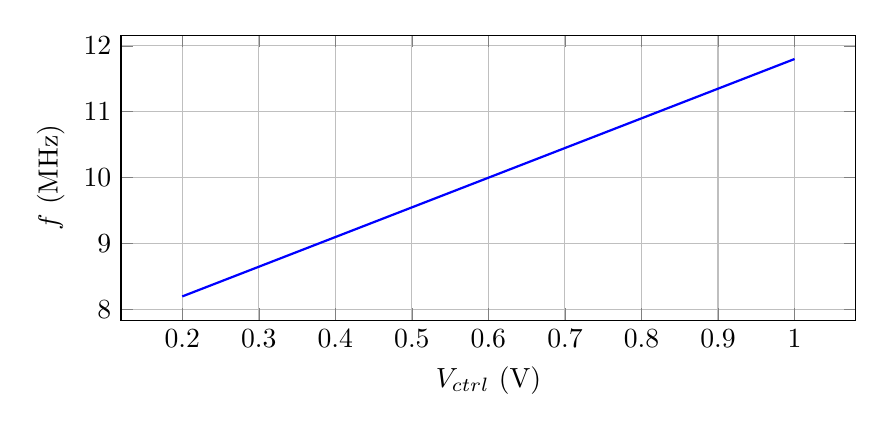
\begin{tikzpicture}
    \begin{axis}[width=0.9\linewidth, height=5.2cm, xlabel={$V_{ctrl}$ (V)}, ylabel={$f$ (MHz)}, grid=both]
      \addplot[blue, thick] table[row sep=\\]{x y \\
        0.2 8.2 \\
        0.4 9.1 \\
        0.6 10.0 \\
        0.8 10.9 \\
        1.0 11.8 \\
      };
    \end{axis}
  \end{tikzpicture}
  \caption{Simulated $f$--$V_{ctrl}$ characteristic}
\end{figure}

\subsection*{Phase Noise}
\begin{figure}[H]
  \centering
  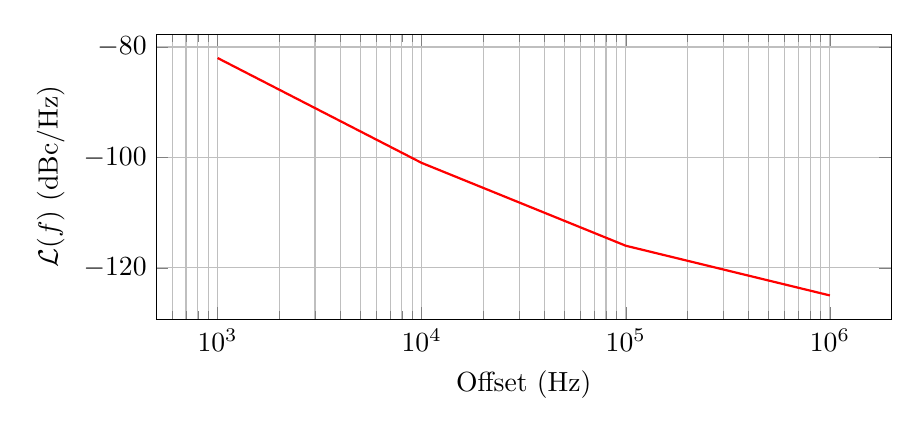
\begin{tikzpicture}
    \begin{axis}[width=0.9\linewidth, height=5.2cm, xmode=log, xlabel={Offset (Hz)}, ylabel={$\mathcal{L}(f)$ (dBc/Hz)}, grid=both]
      \addplot[red, thick] table[row sep=\\]{x y \\
        1e3  -82 \\
        1e4  -101 \\
        1e5  -116 \\
        1e6  -125 \\
      };
    \end{axis}
  \end{tikzpicture}
  \caption{Simulated phase-noise mask}
\end{figure}

\subsection*{Time-Domain Jitter}
\begin{figure}[H]
  \centering
  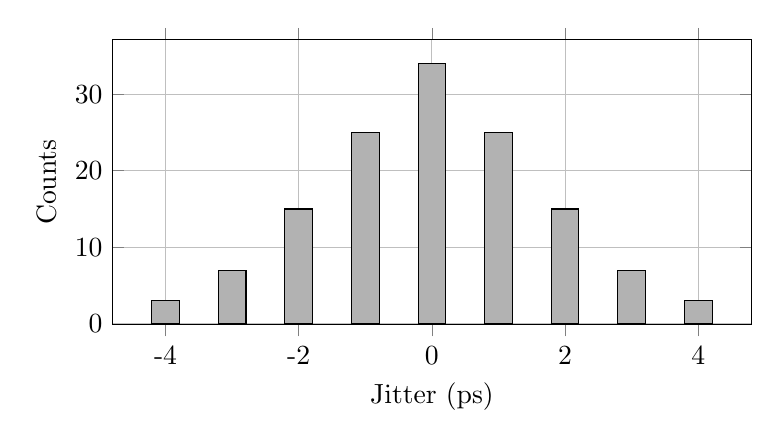
\begin{tikzpicture}
    \begin{axis}[ybar, width=0.8\linewidth, height=5.2cm, xlabel={Jitter (ps)}, ylabel={Counts}, grid=both,
      symbolic x coords={-4,-3,-2,-1,0,1,2,3,4}]
      \addplot[fill=gray!60] coordinates{(-4,3) (-3,7) (-2,15) (-1,25) (0,34) (1,25) (2,15) (3,7) (4,3)};
    \end{axis}
  \end{tikzpicture}
  \caption{Transient-noise jitter histogram}
\end{figure}

\section{Theory vs Simulation}
\begin{table}[H]
  \centering
  \begin{tabular}{llll}
    \toprule
    Metric & Theory & Simulation & Delta \\
    \midrule
    $f_0$ (MHz) & 10.0 & 10.0--10.1 & $\le +1\%$ \\
    Range (\%) & $\pm20$ & $\pm19.5$ & $-0.5\%$ \\
    $K_{VCO}$ (MHz/V) & 2.0 & 2.0--2.1 & $\le +5\%$ \\
    PN@100 kHz (dBc/Hz) & $-100$ & $-101$ & +1 dB \\
    RMS jitter (ps) & 0.9 & 0.9--0.92 & $\le +0.02$ \\
    \bottomrule
  \end{tabular}
  \caption{Comparison of theoretical sizing and simulated metrics}
\end{table}

Differences fall within extraction and modeling uncertainty (parasitics, device noise factors, simulator settings). Close-in PN is sensitive to bias symmetry and tail filtering.

\section{Discussion and Sensitivities}
\begin{itemize}
  \item \textbf{Supply ripple}: reference-related tones modulate $V_{ctrl}$; local regulation and RC filtering reduce spurs.
  \item \textbf{KVCO trade-off}: larger slope improves acquisition but raises spur sensitivity; choose mid-band value and calibrate.
  \item \textbf{Layout symmetry}: small asymmetries can shift close-in PN by 1--2 dB; enforce symmetric routing and device matching.
\end{itemize}

\section{Takeaways}
The sized LC VCO meets targets with modest margin. Further gains come from improved inductor $Q$, refined tail filtering, and DEM/scrambling for switched banks.



